\documentclass[12pt, french]{article}

\usepackage{fancyhdr, fancybox, lastpage,mhchem}
\usepackage[most]{tcolorbox}
\usepackage[a4paper, margin={0.3in, .75in}]{geometry}
\usepackage{wrapfig}
\pagestyle{fancy}
\renewcommand\headrulewidth{1pt}
\renewcommand\footrulewidth{1pt}
\fancyhf{}
\rhead{ \em{Zakaria Haouzan}}
\lhead[C]{\em{2ème année baccalauréat Sciences Physiques}}
\chead[C]{}
\rfoot[C]{}
\lfoot[R]{}
\cfoot[]{\em{Page \thepage / \pageref{LastPage}}}


\newtcolorbox{Box2}[2][]{
                lower separated=false,
                colback=white,
colframe=white!20!black,fonttitle=\bfseries,
colbacktitle=white!30!gray,
coltitle=black,
enhanced,
attach boxed title to top left={yshift=-0.1in,xshift=0.15in},
title=#2,#1}


\begin{document}
\begin{center}
   \shadowbox {\bf{Les transformations liée a
des réactions acides et bases
}
 }

\end{center}

\vspace{-0.2cm}
%%_________________________Exercice ! :"_________________________Exercice
   \begin{Box2}{Exercice 1 :  }
On prépare dans un laboratoire de chimie, une solution
aqueuse d’acide butanoïque $C_3H_7COOH_{(aq)}$ de volume V et de concentration molaire $C = 10^{-2}mol/L$. Le pH de cette solution est : $pH=3,41$.

On modélise la transformation produite par l’équation
chimique suivante: 

\ce{C_3H_7COOH_{(aq)} + H_2O_{(l)} <=> C_3H_7COO^-_{(aq)} + H_3O^+_{(aq)}}

\textbf{1. }Déterminer le taux d’avancement final de la réaction.

\textbf{2. }Trouver, en fonction de C et du pH, l’expression du quotient de réaction $Q_{r,eq}$  à l’équilibre ,puis calculer sa valeur

\textbf{3. }En déduire la valeur du $pK_A$ du couple $C_3H_7COOH/C_3H_7COO^-$


   \end{Box2}


%%_________________________Exercice !2 :"_________________________Exercice
\begin{Box2}{Exercice 2 :}
%\begin{wrapfigure}{r}{0.22\textwidth}
  %\begin{center}
	  %\vspace{-0.6cm}
	%\includegraphics[width=0.22\textwidth]{./img/Ex2.png}
  %\end{center}
%\end{wrapfigure}
Soit une solution aqueuse $(S_a)$ d’acide méthanoique de volume V et de concentration $C_a = 10^{-2}mol/L$. La mesure du pH de cette solution donne $pH=2,9$.

On modélise la transformation chimique qui a lieu entre
l’acide méthanoique et l’eau par l’équation chimique
suivante :

\ce{HCOOH_{(aq)} + H_2O_{(l)} <=> HCOO^-_{(aq)} + H_3O^+_{(aq)}}

\textbf{1. }Dresser le tableau d’avancement de la réaction

\textbf{2. }Montrer que le taux d’avancement final $\tau$ de cette transformation s’écrit sous la forme suivante : $\tau = \frac{10^{-pH}}{C_a}$ calculer $\tau$ et conclure.

\textbf{3. }Déterminer la valeur de la constante $pK_A$ du couple $HCOOH/HCOO^-$

\textbf{4. }On considère une seconde solution aqueuse $(S')$ d'acide propanoïque $C_2H5COOH$ de concentration molaire $C_A =0,010mol/L$.La valeur du taux d'avancement final de la réaction de l'acide propanoïque avec l'eau est $\tau' = 1,16.10^{-1}$

\textbf{4.1. }En comparant t'avec le taux d'avancement final de la
réaction d'acide méthanoïque avec l'eau, indiquer lequel
des deux acides est le plus dissocié en solution.

\textbf{4.2.}Comparer les constantes d'acidité $K_A(HCOOH/HCOO^-)$ et $K(C_2H5COOH/C_2H5COO^-)$ 

\end{Box2}

%%_________________________Exercice ! 3:"_________________________Exercice
\begin{Box2}{Exercice 3 : }
%\begin{wrapfigure}{r}{0.5\textwidth}
  %\begin{center}
	%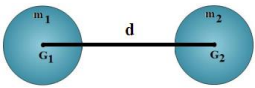
\includegraphics[width=0.5\textwidth]{./img/ex3.png}
  %\end{center}
%\end{wrapfigure}
On dispose d’une solution aqueuse d’acide propanoïque $C_2H5COOH$ de concentration molaire C et de volume V . La mesure du pH de la solution donne la valeur $pH  = 2,9$.

\textbf{1. }Ecrire l’équation modélisant la réaction de l’acide propanoïque avec l’eau.

\textbf{2. }Exprimer le pH de la solution en fonction du $pK_A$ du couple $C_2H5COOH/C_2H5COO^-$ et de la concentration des deux espèces chimiques $C_2H5COO^- $ et $C_2H5COOH$ en solution.

\textbf{3. }Montrer que le taux d’avancement final de la réaction
s’écrit sous la forme : $\tau =  \frac{1}{1 + 10^{pK_A - pH}}$ 
\end{Box2}

%%_________________________Exercice 4 : _________________________Exercice
\begin{Box2}{Exercice 4 : }
   % \begin{wrapfigure}[12]{r}{0.5\textwidth}
  %\begin{center}
	  %\vspace{-0.6cm}
	%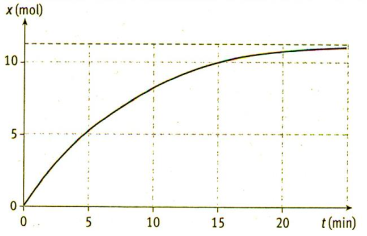
\includegraphics[width=0.5\textwidth]{./img/ex4.png}
  %\end{center}
%\end{wrapfigure}
On considère une solution aqueuse $(S_B)$ d’ammoniaque de volume V et de concentration $C_B$=$2.10^{-2} mol/L$. La mesure de pH de cette solution donne la valeur $pH = 10,75 $ .On donne à $25 ^\circ C$ $pK_e = 14$.

On modélise la transformation chimique qui a lieu entre
l’ammoniaque et l’eau par l’équation chimique suivante :

\ce{NH_{3(aq)} + H_2O_{(l)} <=> NH^{4+}_{(aq)} + HO^-_{(aq)}}

\textbf{1. }Déterminer le taux d’avancement final de cette
réaction . Que peut-on conclure ?

\textbf{2. }Exprimer le quotient de la réaction
$Q_{r,eq}$ ; à l’équilibre du système chimique en fonction de $C_B$ et  $\tau$ . Calculer sa valeur

\textbf{3. }Vérifier la valeur de $pK_A$ du couple $(NH^+_4/NH_3)$
	
\end{Box2}

\vspace{-0.8cm}
\begin{center}
   \Large{ \em{Exercices Supplémentaires}}
\end{center}


\vspace{-0.6cm}
%%_________________________Exercice 5 : _________________________Exercice
\begin{Box2}{Exercice 5 : }
   % \begin{wrapfigure}[14]{r}{0.5\textwidth}
  %\begin{center}
	  %\vspace{-0.6cm}
	%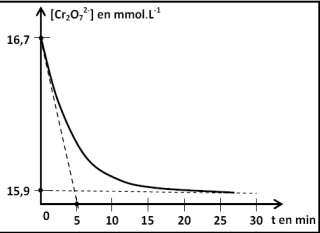
\includegraphics[width=0.5\textwidth]{./img/ex5.png}
  %\end{center}
%\end{wrapfigure}
	Une solution S de méthylamine $\ce{CH_3-NH_2}$ de concentration molaire $C_B = 0,2mol/L$ a un $pH = 12$. On donne à $25^{\circ}C$ $pK_e$ = 14.

	\textbf{1. }Ecrire l’équation de la réaction de l’éthylamine avec l’eau.
	
	\textbf{2. }Calculer les concentrations de toutes les espèces chimiques en solution.

	\textbf{3. }Calculer la constante d’acidité $K_A$ du couple $CH_3NH_3^+/CH_3NH_2$ et son $pK_A$.

\textbf{4. }Tracer le diagramme  de prédominance du couple $CH_3NH_3^+/CH_3NH_2$ En déduire l’espèce prédominante dans la solution S.

\end{Box2}


\begin{Box2}{Exercice 6 : }

	\begin{wrapfigure}[8]{r}{0.34\textwidth}
  \begin{center}
	  \vspace{-0.6cm}
	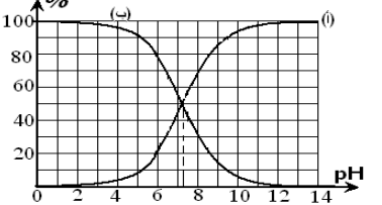
\includegraphics[width=0.34\textwidth]{./img/ex_05.png}
  \end{center}
\end{wrapfigure}
	L’acide hypochloreux a pour formule $HClO_{(aq)}$ . Sa base conjuguée $ClO^-_{(aq)}$ est appelée ion hypochlorite. Le document ci-contre représente les pourcentages des espèces chimiques acide et base du couple $HClO_{aq}/ClO^-_{(aq)}$ en fonction du $pH$ pour une solution

	\textbf{1. }Déterminer graphiquement la valeur numérique de la constante $pK_A$ du couple $HClO_{aq}/ClO^-_{(aq)}$

	\textbf{2. }Laquelle des deux courbes (a) ou (b) correspond à l'hypochlorite? Montre que
 $\%HClO$=$ \frac{[HClO]}{[HClO] + [ClO^-]} = \frac{1}{ 1 + 10^{pH -pK_A}}$
et $\%ClO^-$=$\frac{[ClO^-]}{[HClO] + [ClO^-]}$=$ \frac{1}{ 1 + 10^{pK_A - pH}}$

\textbf{3. }Écrire l'équation de la réaction de $HClO_{(aq)}$
avec de l'eau.

\textbf{4. }On considère une solution d'acide hypochloreux de
$pH=5$ . Déterminer le taux d’avancement de la réaction
dans la solution .
\end{Box2}


\begin{Box2}{Exercice 7 : }
Nous mélangeons $V_1 =20mL$ de solution aqueuse $(S_1)$ d'acide hypochloreux$HClO_{(aq)}$ de concentration $C_1=10^{-2}mol/L$ avec le volume $V_2=10mL$
de solution aqueuse $(S_2)$ d'hydroxyde de sodium de concentration $C_1=C_2$
. On mesure le pH de la solution et on trouve $pH =7,2$ donnée à 25 °C: $pK_e=14$

\textbf{1. }Ecrire l'équation de la réaction de l'acide hypochloreux
avec les ions hydroxyde.

\textbf{2. }montrer que le taux d’avancement de la réaction s’ecrit sous la forme suivante : $\tau = 1-\frac{10^{14 - pH}}{C_2}.\frac{V_1 + V_2}{V_2}$
et calcule sa valeur

\textbf{3. }Exprimer la constante d'équilibre $K$ associée à de la
réaction d'acide hypochloreux et les ions hydroxyde en fonction de $pK_e$ et $pK_A$ constante d'acidité de $HClO_{(aq)}/ClO^-_{(aq)}$, puis calculer leur valeur numérique. 

\end{Box2}


\begin{Box2}{Exercice 8 : }

On mélange dans un volume $V_1$ de la solution aqueuse $S_1$ d’ammoniac
$NH_{3(aq)}$ de concentration Molaire $C_1$ avec un volume $V_1 = V$
d’une solution aqueuse de chlorure de méthyl ammonium $(CH_3NH_{3(aq)^+} ; Cl^-)$ de concentration molaire $C=C_1$

\textbf{1. }Ecrire l’équation chimique modélisant la réaction de
l’ammoniac avec l’ion méthyl ammonium

\textbf{2. }exprime la constante d’équilibre K associée à l’équation de cette réaction en fonction de $pK_{A_1}$ et $pK_{A_2}$ 

\textbf{3. }Montrer que l’expression de la concentration de et celle de dans le mélange réactionnel à l’équilibre,s’écrit $[CH_3NH_{2(aq)}] = [NH_{(aq)}^+]$ = $\frac{C}{2}.\frac{\sqrt{K}}{1+\sqrt{K}}$


\textbf{4. } montre que $pH$ du mélange réactionnel à l’équilibre s’écrit $pH = \frac{1}{2}.(pK_{A_1} + pK_{A_2})$ et calcule sa valeur

$pK_{A1}(NH_4^+/NH_3)=9,2$

$pK_{A2}(CH_3NH_3^+/CH_3NH_2) = 10,7$

\end{Box2}
\end{document}
